\chapter{Appendix material}

\section{Coordinate transformation for a desired line of sight and viewing direction}\label{A:trans}
\begin{figure*}
\centering
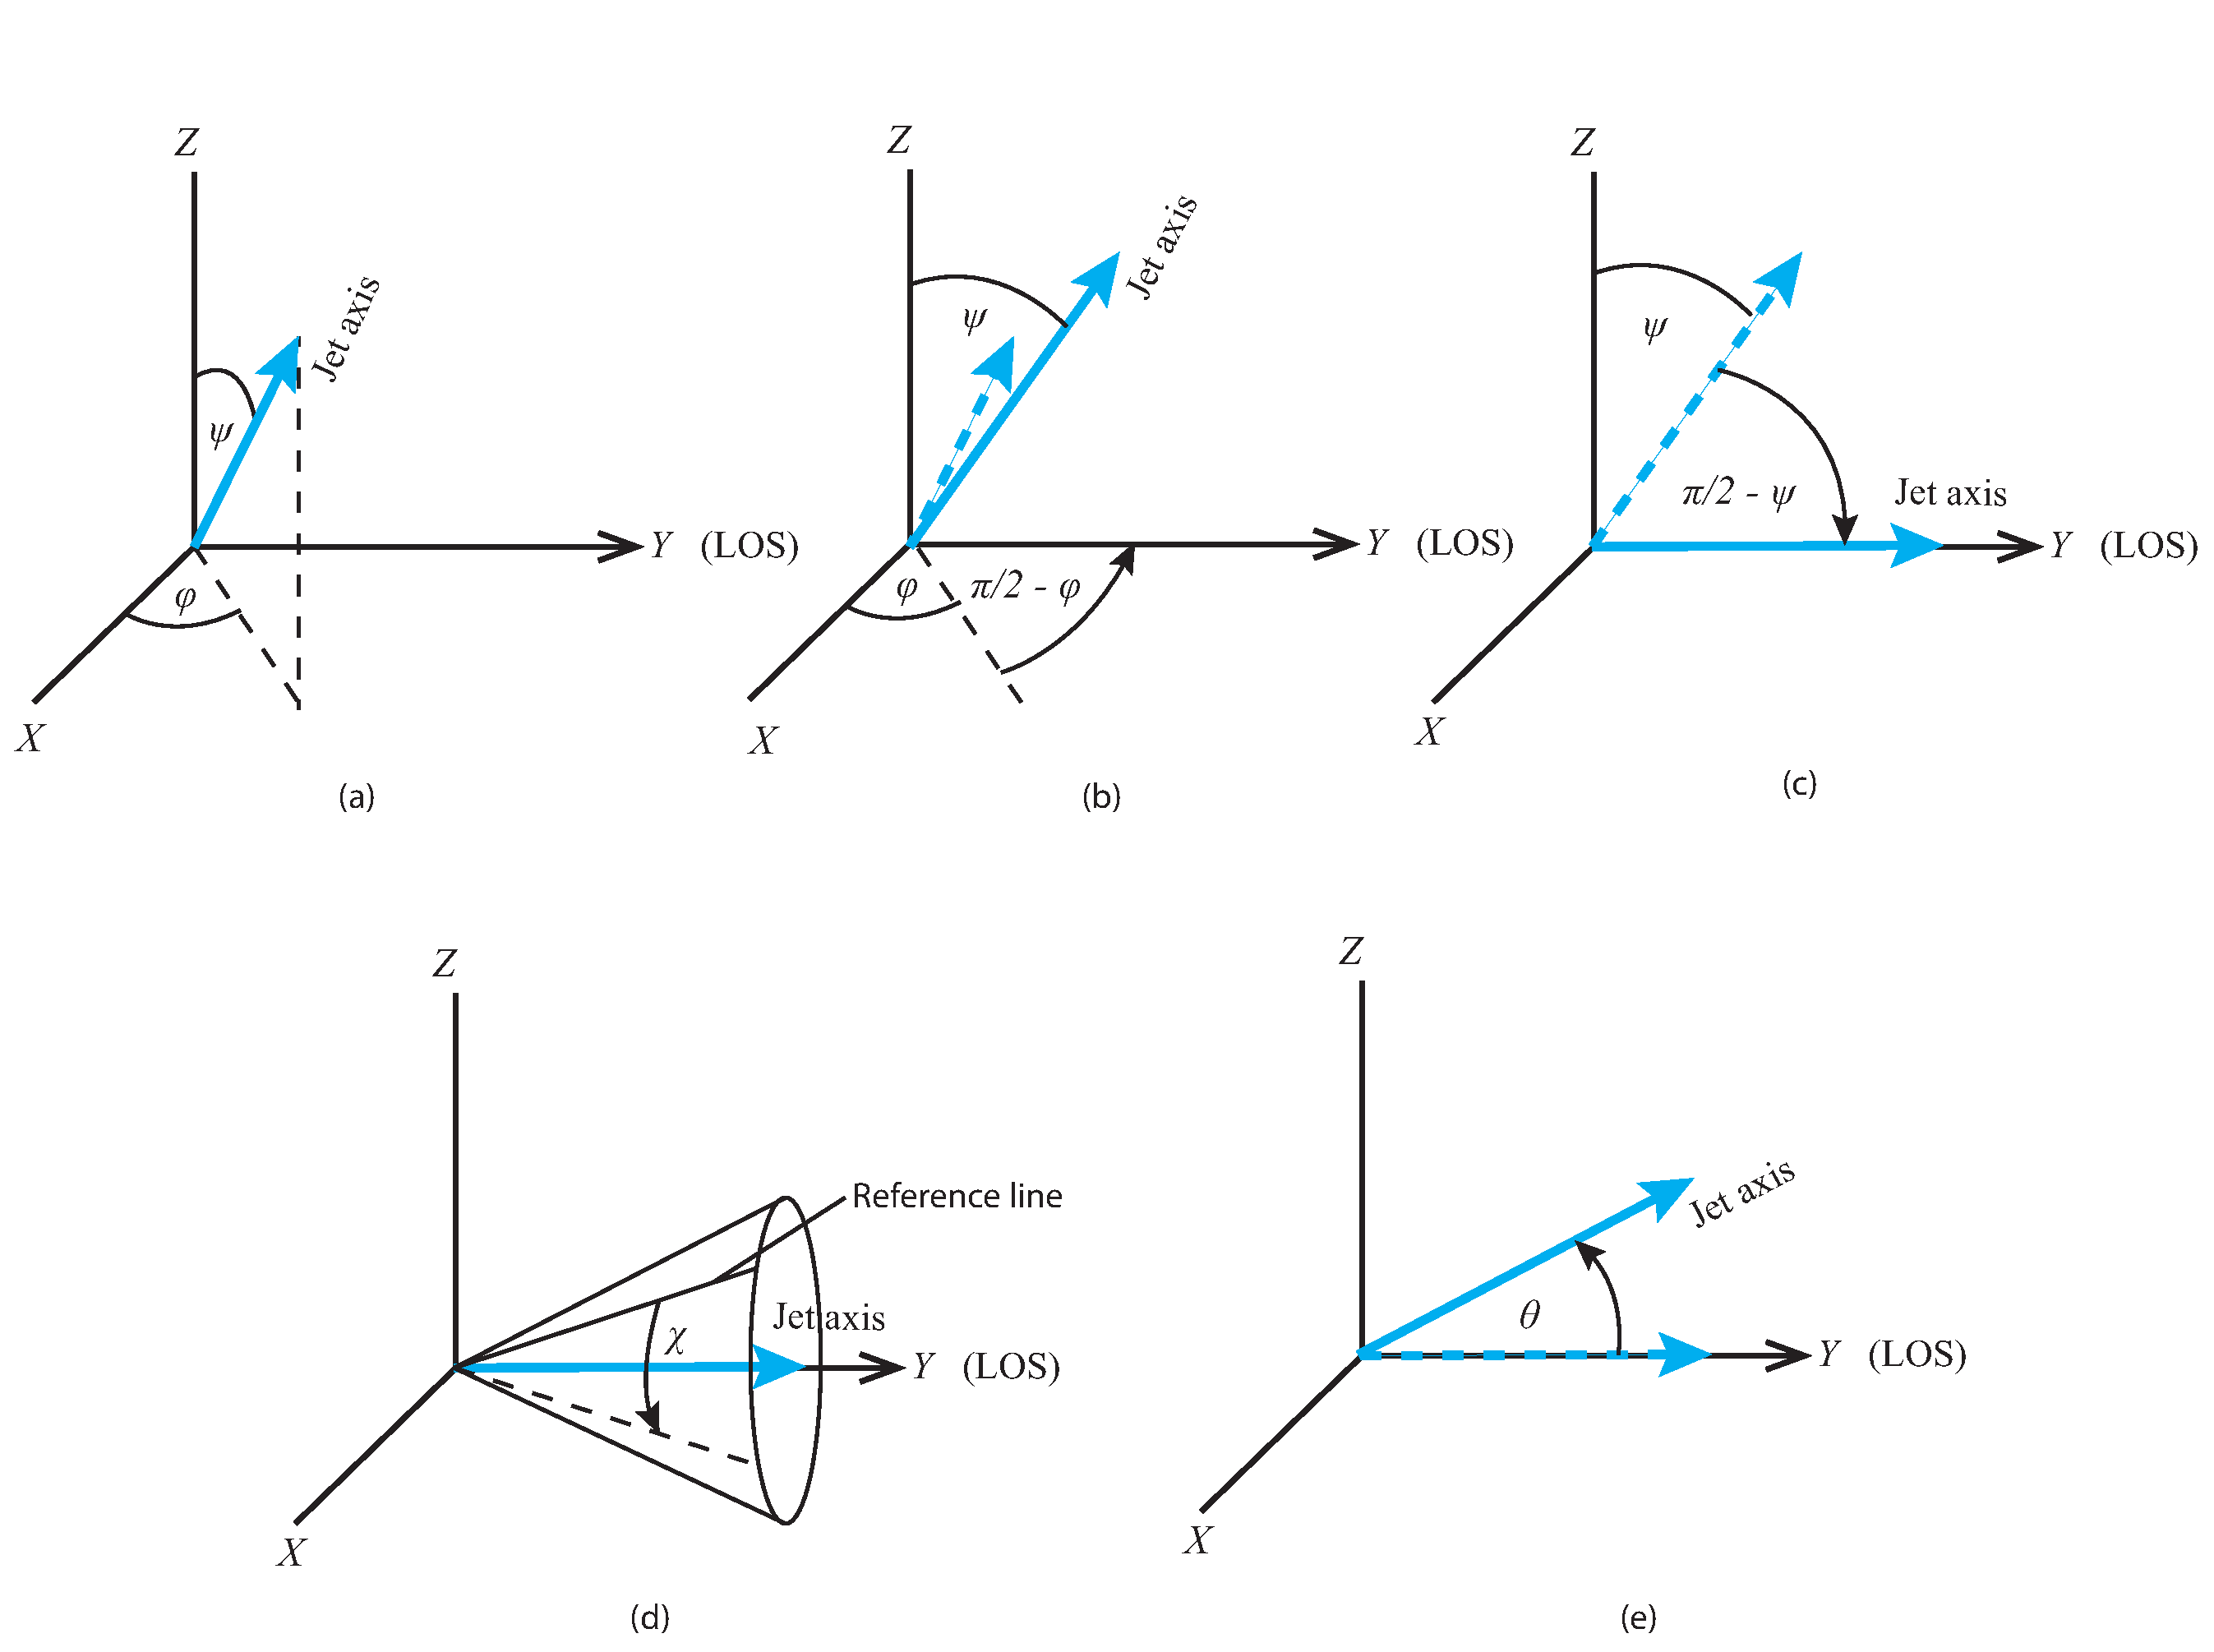
\includegraphics[width=\textwidth]{fig9.eps}
\caption{Transformations of the coordinates associated with the data cube ($xyz$) with respect to coordinates associated with the image cube ($XYZ$) to obtain a line of sight $\theta$ and a viewing direction $\chi$. The line of sight is along the $Y$ axis. See text in Appendix~\ref{A:trans} for details.  }
\label{f:rot}
\end{figure*}
Let $xyz$ be the coordinates (shown in panel (a) of Fig.~\ref{f:rot}) associated with the simulation data cube. At a given time the jet (shown in a blue thick line in panel (a)) makes angles $\psi$ and $\phi$ with the $z$ and $x$ axes. Let $XYZ$ be the coordinates (shown in panel (a) of Fig.~\ref{f:rot}) associated with the synthetic image cube. 
To obtain a desired line of sight and viewing direction we perform the following rotations of the simulation data cube with respect to the synthetic image cube. These rotations are depicted in Fig.~\ref{f:rot}. In each panels of this figure the coordinates associated with the image cubes are shown in bold solid lines, the coordinates associated with the simulation data cubes are in solid (before transformations) and dashed (after transformations) lines, the jets before transformations are in light blue thick lines and the jet after transformations are in dark blue thick lines. 
\begin{enumerate}
\item First we rotate the simulation data cube (anticlockwise) with respect to the $Z$-axis by an angle $\pi/2 - \phi$ (shown in (a)). The coordinates associated with the simulation data cube $xyz$ are transformed to $x'y'z'$. This rotation brings the jet on the $YZ$ plane. The rotation matrix for this rotation $R^{(AC)}_{Z(\pi/2 - \phi)}$ (here the superscript AC denotes the anticlockwise rotation) is given by 
\begin{eqnarray}
R^{(AC)}_{Z(\pi/2 - \phi)}  &=& \begin{pmatrix}
 \cos(\pi/2 - \phi) & -\sin(\pi/2 - \phi) & 0 \\
\sin(\pi/2 - \phi) & \cos(\pi/2 - \phi) & 0 \\
0 & 0 & 1
\end{pmatrix} \nonumber \\
&=& \begin{pmatrix}
 \sin\phi & -\cos\phi & 0 \\
\cos\phi & \sin\phi & 0 \\
0 & 0 & 1
\end{pmatrix} 
\end{eqnarray}
\item We rotate the simulation data cube second time (clockwise) with respect to the $X$-axis by an angle $\pi/2 - \theta$ (shown in panel (b)). The coordinates associated with the simulation data cube $x'y'z'$ are transformed to $x''y''z''$. This rotation makes the jet axis aligned with the line of sight $Y$-axis. The rotation matrix for this rotation $R^{(C)}_{X(\pi/2 - \psi)}$ (the superscript C denotes the clockwise rotation) is given by 
\begin{eqnarray}
R^{(C)}_{X(\pi/2 - \psi)} &=& \begin{pmatrix}
 1 & 0 & 0 \\
0 & \cos(\pi/2 - \psi) & \sin(\pi/2 - \psi) \\
0 & -\sin(\pi/2 - \psi) & \cos(\pi/2 - \psi)
\end{pmatrix} \nonumber \\
& = &\begin{pmatrix}
1 & 0 & 0 \\
0 & \sin\psi & \cos\psi \\
0 & -\cos\psi & \sin\psi
\end{pmatrix}  
\end{eqnarray}
\item Now to obtain a viewing direction we rotate the simulation data cube with respect to the $Y$-axis by an angle $\chi$ (shown in panel (c)). The coordinates associated with the simulation data cube $x''y''z''$ are transformed to $x'''y'''z'''$. The rotation matrix for this rotation $R^{(AC)}_{Y(\chi)} $ is given by
\begin{equation}
R^{(AC)}_{Y(\chi)} = \begin{pmatrix}
 \cos\chi & 0 & \sin\chi \\
0 & 1  & 0 \\
-\sin\chi & 0 & \cos\chi
\end{pmatrix}  
\end{equation}
\item Finally, we rotate the simulation data cube with respect to the $X$-axis by and angle $\theta$ (shown in panel (d)). This rotation relocates the jet (shown in dark blue thick line) at an angle $\theta$ with respect to the $Y$-axis (line of sight). The coordinates associated with the simulation data cube $x'''y'''z'''$ are transformed to $x''''y''''z''''$. The rotation matrix associated with this rotation $R'^{(AC)}_{X(\theta)}$ is given by
 \begin{equation}
  R'^{(AC)}_{X(\theta)} = \begin{pmatrix}
 1 & 0 & 0 \\
0 & \cos\theta & -\sin\theta \\
0 & \sin\theta & \cos\theta 
\end{pmatrix}  
\end{equation}
\end{enumerate} 

The velocity of the fluid in the synthetic image cube $\textbf{v}'$ after the transformations described above is estimated from the velocity in the simulation data cube by using the rotation matrix $R = R'^{(AC)}_{X(\theta)} R^{(AC)}_{Y(\chi)} R^{(C)}_{X(\pi/2 - \psi)} R^{(AC)}_{Z(\pi/2 - \phi)}$
\begin{equation}
\textbf{v}' = R \textbf{v}
\end{equation}

Let $s_1 = \sin \psi$, $s_2 = \sin \phi$, $s_3 = \sin \chi$, $s_4 = \sin \theta$, $c_1 = \cos \psi$,  $c_2 = \cos \phi$, $c_3 = \cos \chi$, and $c_4 = \cos\theta$. Then the rotation matrix $R$ is given by:
 \begin{eqnarray}
  R &=&  R'^{(AC)}_{X(\theta)} R^{(AC)}_{Y(\chi)} R^{(C)}_{X(\pi/2 - \psi)} R^{(AC)}_{Z(\pi/2 - \phi)} \nonumber \\
  &=&  \begin{pmatrix}
  c_3 s_2 - s_3 c_1 c_2  & -c_3 c_2 -s_3 c_1 s_2 & s_3 s_1 \\[6pt]
  c_4 s_1 c_2 + s_4 s_3 s_2  &  c_4 s_1 s_2 + s_4 s_3 c_2 & c_4 c_1 - s_4 c_3 s_1  \\
\phantom{{}+{}}+ s_4 c_3 c_1 c_2 & \phantom{{}+{}}- s_4 c_3 c_1 s_2  & & \\[6pt]
   s_4 s_1 c_2 - c_4 s_3 s_2 & s_4 s_1 s_2 + c_4 s_3 c_2  &  s_4 c_1 + c_4 c_3 s_1 \\
\phantom{{}+{}} - c_4 c_3 c_1c_2   &\phantom{{}+{}}-c_4 c_3 c_1 s_2  & & \\
\end{pmatrix} \nonumber 
\end{eqnarray}

% \begin{eqnarray}
%  R &=&  R'^{(AC)}_{X(\theta)} R^{(AC)}_{Y(\chi)} R^{(C)}_{X(\pi/2 - \psi)} R^{(AC)}_{Z(\pi/2 - \phi)} \nonumber \\
%  &=&  \begin{pmatrix}
%  c\chi s\phi - s\chi c\psi c\phi  & -c\chi c\phi -s\chi c\psi s\phi & s\chi s\psi \\[6pt]
%  c\theta s\psi c\phi + s\theta s\chi s\phi  &  c\theta s\psi s\phi + s\theta s\chi c\phi & c\theta c\psi - s\theta c\chi s\psi  \\
%\phantom{{}+{}+{}}+ s\theta c\chi c\psi c\phi & \phantom{{}+{}+{}}- s\theta c\chi c\psi s\phi  & & \\[6pt]
%   s\theta s\psi c\phi - c\theta s\chi s\phi & s\theta s\psi s\phi + c\theta s\chi c\phi  &  s\theta c\psi + c\theta c\chi s\psi \\
%\phantom{{}+{}+{}} - c\theta c\chi c\psi c\phi   &\phantom{{}+{}+{}}-c\theta c\chi c\psi s\phi  & & \\
%\end{pmatrix} \nonumber 
%\end{eqnarray}

%where $s$ and $c$ stands for $\sin$ and $\cos$ respectively. 

% \cos\chi \sin\phi - \sin\chi \cos\psi \cos\phi  & -\cos\chi \cos\phi -\sin\chi \cos\psi \sin\phi & \sin\chi \sin\psi \\

\section{Synthetic surface brightness of the source at different $\theta$ and $\chi$}\label{A:morph}
\begin{figure*}
\centering
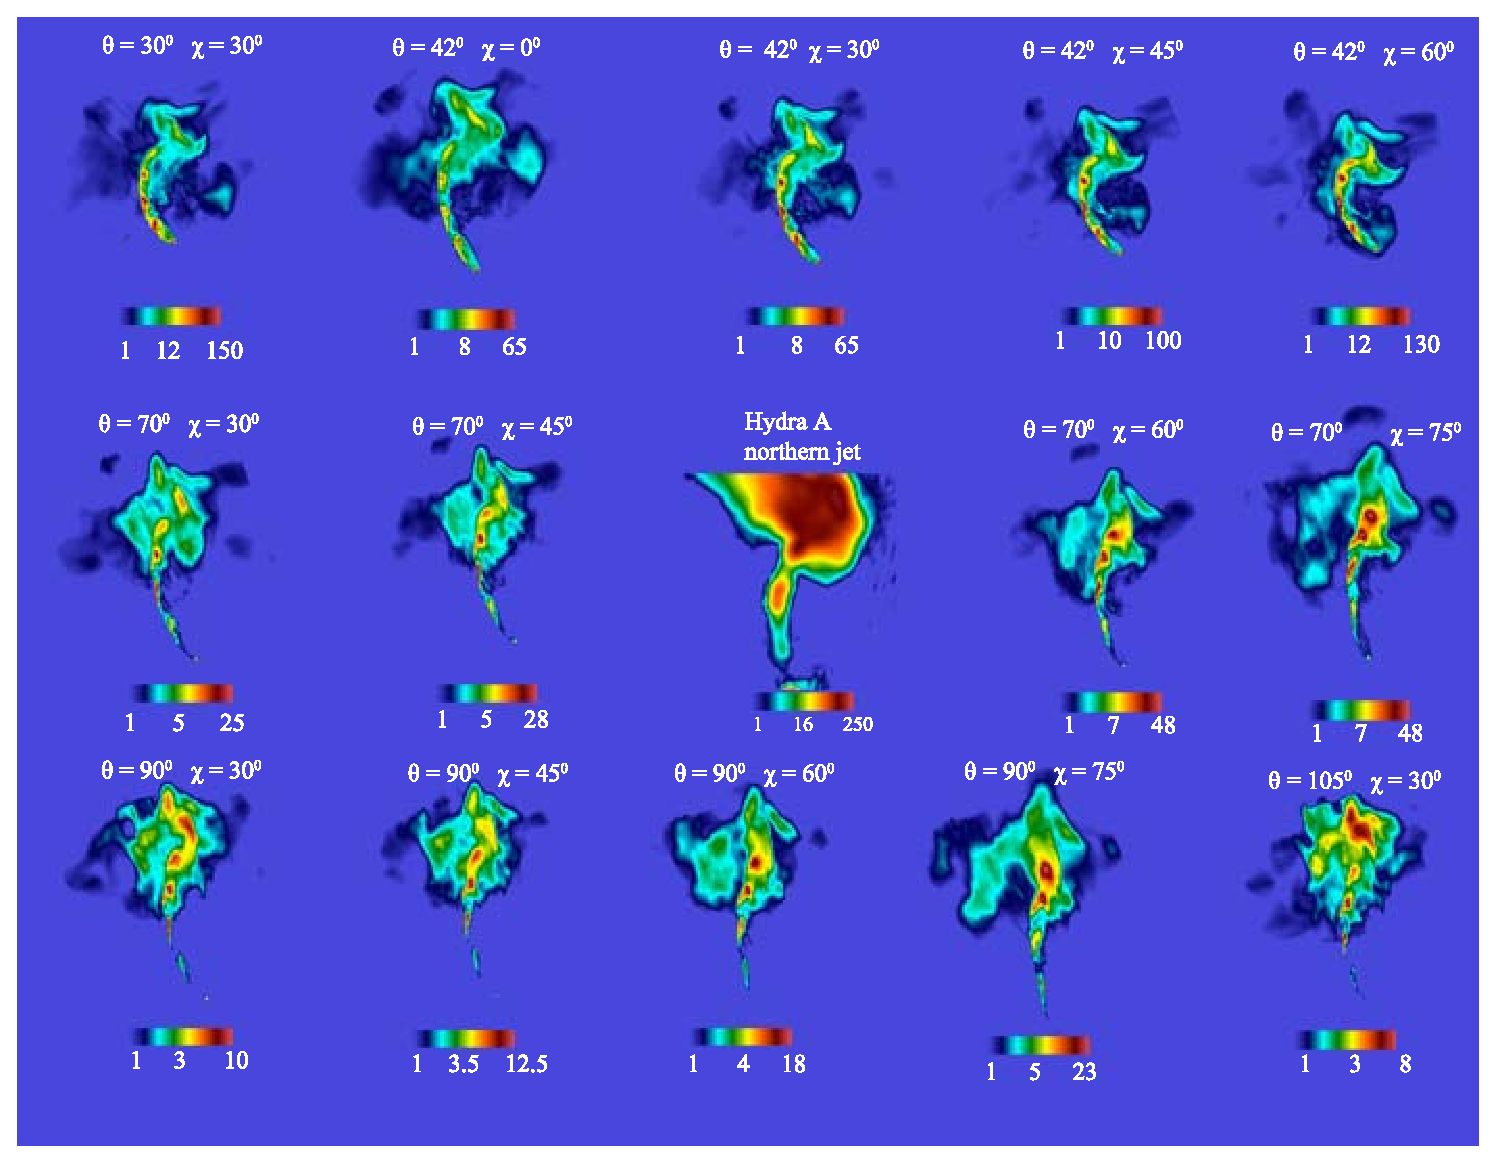
\includegraphics[width=\textwidth]{fig10.eps}
\caption{ Synthetic surface brightness images of the best match model for different line of sights $\theta$ and viewing directions $\chi$. For comparison the observed radio image of the inner 20~kpc of the Hydra A northern jet is shown at the third column of second row. }
\label{f:morph}
\end{figure*}






































%\section{Table~\ref{table:Sayurirrab}}
%

%A cross-match between the current data set and that of \citet{prior09} confirmed four objects as RRab. Of these, two were previously identified as undefined variables, one as non-variable and the other one as RRc. Object 116385.432 was identified as RRab by \citet{prior09}. We find this star as a Blazhko RRab as we have two sets of observations separated by $\sim100$ days. These are given in Table~\ref{table:Sayurirrab}. While calculating the completeness profiles, these objects were considered as RRab (Sections~\ref{s3.3} and ~\ref{s5}).
%
%\section{Table~\ref{table:fromSayuri}}
%
%This table presents two objects that were confirmed as RRLs by \citet{prior09}, but could not be identified in this study due to insufficient observations. A third object 115213.329 is clarified as RRab with the help of \citet{prior09}'s catalog. We found the same period. However, we could not confirm the amplitude as we need more observations. We considered these three objects as RRLs in the completeness profile calculations, though we could not calibrate them photometrically.
%
%\ctable[sideways,cap=Objects Reidentified by Current Study from \citet{prior09},caption=Objects Reidentified by Current Study from \citet{prior09},label=table:Sayurirrab,doinside=\normalsize \setlength{\extrarowheight}{2pt}
%,captionskip=3pt]{lccccccccccc}
%{\tnote[a]{Found by current study.}
%\tnote[b]{Confirmed by \citet{prior09}.}
%\tnote[c]{Undefined variables.}
%\tnote[d]{Non-variables.}
%} 
%{\toprule[2pt]
%Star ID & R.A. & Decl. & $V_{\rm{SEKBO}}$ & $N_{\rm{Obs}}\tmark[a]$ & $N_{\rm{Obs}}\tmark[b]$ & Star Type\tmark[a] & Star Type\tmark[b] & Period\tmark[a] & Period\tmark[b] & $A_{\rm{V}}\tmark[a]$ &$A_{\rm{V}}\tmark[b]$\\
%& (J2000.0) & (J2000.0) & & & & &  & (days) & (days) & & \\
%\midrule
%116709.1029 & 03 29 23.66 & 16 37 52.33 & 17.58 & 08 & 09 & RRab & UV\tmark[c] & 0.603 & ... & 0.742 & ...\\
%110735.919 & 21 14 25.80 & $-13 57 27.62$ & 17.42 & 16 & 12 & RRab & NV\tmark[d] & 0.516 & ... & 0.955 & ...\\
%125812.515 & 21 48 49.46 & $-16 49 53.14$ & 17.28 & 13 & 05 & RRab & UV\tmark[c] & 0.595 & ... & 0.818 & ... \\
%127806.438 & 00 25 23.38 & $-03 15 22.88$ & 17.24 & 07 & 06 & RRab & RRc & 0.597 & 0.286 & 0.743 & 0.358\\
%116385.432 & 02 10 44.39 & 12 45 09.71 & 17.88 & 09 & 08 & Blazhko RRab & RRab & 0.547 & 0.547 & 0.605 & 0.641\\
%\addlinespace[5pt]\bottomrule[2pt]}
%
%\ctable[sideways,cap=Objects Identified from \citet{prior09},caption=Objects Identified from \citet{prior09},label=table:fromSayuri,doinside=\normalsize \setlength{\extrarowheight}{2pt}
%,captionskip=3pt]{lccccccccccc}
%{\tnote[a]{Confirmed by \citet{prior09}.}
%\tnote[b]{Found by current study.}
%\tnote[c]{Non-variables.}
%} 
%{\toprule[2pt]
%Star ID & R.A. & Decl. & $V_{\rm{SEKBO}}$ & $N_{\rm{Obs}}\tmark[a]$ & $N_{\rm{Obs}}\tmark[b]$ & Star Type$\tmark[a]$ & Star Type$\tmark[b]$ & Period$\tmark[a]$ & Period$\tmark[b]$ & $A_{\rm{V}}\tmark[a]$ & $A_{\rm{V}}\tmark[b]$\\
% & (J2000.0) & (J2000.0) &  &  &  &  &  & (days) & (days) &  &\\
%\midrule
%101751.216 & 02 11 41.33 & 03 29 41.10 & 15.03 & 09 & 06 & RRc & NV\tmark[c] & 0.347 & ... & 0.377 & ...\\
%104410.220 & 03 19 04.26 & 09 14 20.32 & 15.13 & 09 & 09 & RRab & NV\tmark[c] & 0.664 & ... & 0.590 & ...\\
%115213.329 & 03 23 36.23 & 14 47 54.25 & 15.50 & 12 & 05 & RRab & RRab & 0.625 & 0.625 & 0.505 & ...\\
%\addlinespace[5pt]\bottomrule[2pt]}
%
%\section{Light Curves}
%
%Figure~\ref{fig:finallc} shows the final light curves for the confirmed RRLs (43 RRab and 11 RRc). RRLs showing the Blazhko effect are noted with an asterisk following the variable name.
%
%\begin{figure}[ht]
%\begin{minipage}[b]{0.3\linewidth}
%\centering
%\includegraphics[scale=0.25]{f11_1.pdf}%1
%\end{minipage}
%\begin{minipage}[b]{0.3\linewidth}
%\centering
%\includegraphics[scale=0.25]{f11_2.pdf}%2
%\end{minipage}
%\begin{minipage}[b]{0.3\linewidth}
%\centering
%\includegraphics[scale=0.25]{f11_3.pdf}%3
%\end{minipage}
%\begin{minipage}[b]{0.3\linewidth}
%\centering
%\includegraphics[scale=0.25]{f11_4.pdf}%4
%\end{minipage}
%\begin{minipage}[b]{0.3\linewidth}
%\centering
%\includegraphics[scale=0.25]{f11_5.pdf}%5
%\end{minipage}
%\begin{minipage}[b]{0.3\linewidth}
%\centering
%\includegraphics[scale=0.25]{f11_6.pdf}%6
%\end{minipage}
%\begin{minipage}[b]{0.3\linewidth}
%\centering
%\includegraphics[scale=0.25]{f11_7.pdf}%7
%\end{minipage}
%\begin{minipage}[b]{0.3\linewidth}
%\centering
%\includegraphics[scale=0.25]{f11_8.pdf}%8
%\end{minipage}
%\begin{minipage}[b]{0.3\linewidth}
%\centering
%\includegraphics[scale=0.25]{f11_9.pdf}%9
%\end{minipage}
%\begin{minipage}[b]{0.3\linewidth}
%\centering
%\includegraphics[scale=0.25]{f11_10.pdf}%10
%\end{minipage}
%\hspace{0.54cm}
%\begin{minipage}[b]{0.3\linewidth}
%\centering
%\includegraphics[scale=0.25]{f11_11.pdf}%11
%\end{minipage}
%\hspace{0.54cm}
%\begin{minipage}[b]{0.3\linewidth}
%\centering
%\includegraphics[scale=0.25]{f11_12.pdf}%12
%\end{minipage}
%\end{figure}
%\begin{figure}
%%%\clearpage
%\begin{minipage}[b]{0.3\linewidth}
%\centering
%\includegraphics[scale=0.25]{f11_13.pdf}%13
%\end{minipage}
%\begin{minipage}[b]{0.3\linewidth}
%\centering
%\includegraphics[scale=0.25]{f11_14.pdf}%14
%\end{minipage}
%\begin{minipage}[b]{0.3\linewidth}
%\centering
%\includegraphics[scale=0.25]{f11_15.pdf}%15
%\end{minipage}
%\begin{minipage}[b]{0.3\linewidth}
%\centering
%\includegraphics[scale=0.25]{f11_16.pdf}%16
%\end{minipage}
%\begin{minipage}[b]{0.3\linewidth}
%\centering
%\includegraphics[scale=0.25]{f11_17.pdf}%17
%\end{minipage}
%\begin{minipage}[b]{0.3\linewidth}
%\centering
%\includegraphics[scale=0.25]{f11_18.pdf}%18
%\end{minipage}
%\begin{minipage}[b]{0.3\linewidth}
%\centering
%\includegraphics[scale=0.25]{f11_19.pdf}%19
%\end{minipage}
%\begin{minipage}[b]{0.3\linewidth}
%\centering
%\includegraphics[scale=0.25]{f11_20.pdf}%20
%\end{minipage}
%\begin{minipage}[b]{0.3\linewidth}
%\centering
%\includegraphics[scale=0.25]{f11_21.pdf}%21
%\end{minipage}
%\begin{minipage}[b]{0.3\linewidth}
%\centering
%\includegraphics[scale=0.25]{f11_22.pdf}%22
%\end{minipage}
%\begin{minipage}[b]{0.3\linewidth}
%\centering
%\includegraphics[scale=0.25]{f11_23.pdf}%23
%\end{minipage}
%\begin{minipage}[b]{0.3\linewidth}
%\centering
%\includegraphics[scale=0.25]{f11_24.pdf}%24
%\end{minipage}
%\begin{minipage}[b]{0.3\linewidth}
%\centering
%\includegraphics[scale=0.25]{f11_25.pdf}%25
%\end{minipage}
%\hspace{0.54cm}
%\begin{minipage}[b]{0.3\linewidth}
%\centering
%\includegraphics[scale=0.25]{f11_26.pdf}%26
%\end{minipage}
%\hspace{0.54cm}
%\begin{minipage}[b]{0.3\linewidth}
%\centering
%\includegraphics[scale=0.25]{f11_27.pdf}%27
%\end{minipage}
%\end{figure}
%\begin{figure}
%\begin{minipage}[b]{0.3\linewidth}
%\centering
%\includegraphics[scale=0.25]{f11_28.pdf}%28
%\end{minipage}
%\begin{minipage}[b]{0.3\linewidth}
%\centering
%\includegraphics[scale=0.25]{f11_29.pdf}%29
%\end{minipage}
%\begin{minipage}[b]{0.3\linewidth}
%\centering
%\includegraphics[scale=0.25]{f11_30.pdf}%30
%\end{minipage}
%\begin{minipage}[b]{0.3\linewidth}
%\centering
%\includegraphics[scale=0.25]{f11_31.pdf}%31
%\end{minipage}
%\begin{minipage}[b]{0.3\linewidth}
%\centering
%\includegraphics[scale=0.25]{f11_32.pdf}%32
%\end{minipage}
%\begin{minipage}[b]{0.3\linewidth}
%\centering
%\includegraphics[scale=0.25]{f11_33.pdf}%33
%\end{minipage}
%\begin{minipage}[b]{0.3\linewidth}
%\centering
%\includegraphics[scale=0.25]{f11_34.pdf}%34
%\end{minipage}
%\begin{minipage}[b]{0.3\linewidth}
%\centering
%\includegraphics[scale=0.25]{f11_35.pdf}%35
%\end{minipage}
%\begin{minipage}[b]{0.3\linewidth}
%\centering
%\includegraphics[scale=0.25]{f11_36.pdf}%36
%\end{minipage}
%\begin{minipage}[b]{0.3\linewidth}
%\centering
%\includegraphics[scale=0.25]{f11_37.pdf}%37
%\end{minipage}
%\begin{minipage}[b]{0.3\linewidth}
%\centering
%\includegraphics[scale=0.25]{f11_38.pdf}%38
%\end{minipage}
%\begin{minipage}[b]{0.3\linewidth}
%\centering
%\includegraphics[scale=0.25]{f11_39.pdf}%39
%\end{minipage}
%\begin{minipage}[b]{0.3\linewidth}
%\centering
%\includegraphics[scale=0.25]{f11_40.pdf}%40
%\end{minipage}
%\hspace{0.54cm}
%\begin{minipage}[b]{0.3\linewidth}
%\centering
%\includegraphics[scale=0.25]{f11_41.pdf}%41
%\end{minipage}
%\hspace{0.54cm}
%\begin{minipage}[b]{0.3\linewidth}
%\centering
%\includegraphics[scale=0.25]{f11_42.pdf}%42
%\end{minipage}
%\end{figure}
%\begin{figure}
%\begin{minipage}[b]{0.3\linewidth}
%\centering
%\includegraphics[scale=0.25]{f11_43.pdf}%43
%\end{minipage}
%\begin{minipage}[b]{0.3\linewidth}
%\centering
%\includegraphics[scale=0.25]{f11_44.pdf}%44
%\end{minipage}
%\begin{minipage}[b]{0.3\linewidth}
%\centering
%\includegraphics[scale=0.25]{f11_45.pdf}%45
%\end{minipage}
%\begin{minipage}[b]{0.3\linewidth}
%\centering
%\includegraphics[scale=0.25]{f11_46.pdf}%46
%\end{minipage}
%\begin{minipage}[b]{0.3\linewidth}
%\centering
%\includegraphics[scale=0.25]{f11_47.pdf}%47
%\end{minipage}
%\begin{minipage}[b]{0.3\linewidth}
%\centering
%\includegraphics[scale=0.25]{f11_48.pdf}%48
%\end{minipage}
%\begin{minipage}[b]{0.3\linewidth}
%\centering
%\includegraphics[scale=0.25]{f11_49.pdf}%49
%\end{minipage}
%\begin{minipage}[b]{0.3\linewidth}
%\centering
%\includegraphics[scale=0.25]{f11_50.pdf}%50
%\end{minipage}
%\begin{minipage}[b]{0.3\linewidth}
%\centering
%\includegraphics[scale=0.25]{f11_51.pdf}%51
%\end{minipage}
%\begin{minipage}[b]{0.3\linewidth}
%\centering
%\includegraphics[scale=0.25]{f11_52.pdf}%52
%\end{minipage}
%\hspace{0.54cm}
%\begin{minipage}[b]{0.3\linewidth}
%\centering
%\includegraphics[scale=0.25]{f11_53.pdf}%53
%\end{minipage}
%\hspace{0.54cm}
%\begin{minipage}[b]{0.3\linewidth}
%\centering
%\includegraphics[scale=0.25]{f11_54.pdf}%54
%\end{minipage}
%\caption[Final light curves for confirmed RR Lyraes (43 RRab and 11 RRc)]{Final light curves for confirmed RR Lyraes (43 RRab and 11 RRc). Plots with $"*"$ are indicating Blazhko RRLs.}
%\label{fig:finallc}
%\end{figure}
%
%\ctable[caption=Positions and Derived Parameters for Confirmed RR Lyraes,doinside=\scriptsize,pos=p,captionskip=3pt,width=1.05\textwidth,label=table:all]{lccccccccccc}
%{\tnote[a]{Found by current study.}
%\tnote[b]{Confirmed by \citet{prior09}.}
%}
%{
%\toprule[2pt]
%Star ID & R.A. & Decl. & Star & $N_{\rm{Obs}}$ & $V_{\rm{SEKBO}}$ & $V_{\rm{FT}}$ & $V_{\rm{Diff}}$ & Per\tmark[a] & $A_{\rm{V}}\tmark[a]$ & Per\tmark[b] & $A_{\rm{V}}\tmark[b]$\\
%& (J2000.0) & (J2000.0) & Type & & & & & (days) & & (days) &\\
%\midrule
%127806.85 & 00 25 12.59 & $-$03 31 29.75 & RRab & 06 & 17.22 & 17.519 & $$-$0.299$ & 0.519 & 0.866 & 0.643 & 1.183\\
%127806.438 & 00 25 23.38 & $-$03 15 22.88 & RRab & 07 & 17.24 & 17.397 & $$-$0.157$ & 0.597 & 0.743 & 0.286 & 0.358\\
%127102.361 & 00 45 22.49 & $-$04 31 58.99 & RRab & 14 & 17.78 & 17.669 & 0.111 & 0.567 & 0.754 & &\\           
%103340.519 & 01 40 20.19 & 08 44 01.17 & RRab & 08 & 17.39 & 17.363 & 0.027 & 0.554 & 0.893 & &\\           
%116383.660 & 01 49 51.64 & 10 55 11.86 & RRc & 14 & 18.10 & 18.200 & $-$0.100 & 0.342 & 0.520 & &\\
%116385.432 & 02 10 44.39 & 12 45 09.71 & RRab & 09 & 17.88 & 18.284 & $-$0.404 & 0.547 & 0.605 & 0.547 & 0.641\\
%101751.216 & 02 11 41.33 & 03 29 41.10 & RRc & 06 & 15.03 &  &  & 0.347& 0.377 & 0.347 & 0.377\\
%116920.426 & 02 12 42.68 & 11 19 57.14 & RRab & 15 & 17.90 & 17.878 & 0.022 & 0.574 & 0.761 & 0.575 &0.554\\
%129320.530 & 02 31 01.07 & 11 42 47.68 & RRab & 08 & 18.14 & 18.265 & $-$0.125 & 0.623 & 0.727  & &\\
%104410.220 & 03 19 04.26 & 09 14 20.32 & RRab & 09 & 15.13 &  & & 0.664 & 0.590 & 0.664 & 0.590\\
%104410.181 & 03 19 05.03 & 09 08 41.95 & RRab & 10 & 17.00 & 17.362 & $-$0.362 & 0.544 & 0.815 & 0.544 & 0.587\\
%115511.269 & 03 22 28.88 & 13 30 59.29 & RRab & 06 & 16.74 & 17.035 & $-$0.295 & 0.531 & 0.571 & 0.531 & 0.571\\
%115213.329 & 03 23 36.23 & 14 47 54.25 & RRab & 05 & 15.50  & & & 0.625 & 0.505 & 0.625 & 0.505\\
%116709.1029 & 03 29 23.66 & 16 37 52.33 & RRab & 08 & 17.58 & 17.866 & $-$0.286 & 0.603 & 0.742 & &\\
%103170.1054 & 03 49 11.45 & 18 06 30.01 & RRab & 07 & 18.66 & 18.923 & $-$0.263 & 0.619 & 0.693 & &\\
%103815.292 & 04 26 16.31 & 19 10 54.97 & RRab & 06 & 16.57 & 16.995 & $-$0.425 & 0.593 & 0.842 & &\\
%104638.2589 & 07 37 32.34 & 11 15 51.86 & RRab & 27 & 19.09 & 18.958  & 0.132 & 0.523 & 1.117 & 0.521 & 1.169\\
%104812.1840 & 07 40 00.37 & 11 44 04.49 & RRab & 15 & 18.60 & 18.712 & $-$0.112 & 0.622 & 0.790 & &\\
%117602.795 & 07 54 14.74 & 15 05 23.31 & RRab & 18 & 15.34 & 15.197 & 0.143 & 0.525 & 0.809 & &\\
%109614.1159 & 13 20 46.75 & $-$05 42 34.73 & RRab & 11 & 19.07 & 19.163 & $-$0.093 & 0.617 & 0.777 & &\\
%97894.1051 & 13 44 01.99 & $-$10 56 53.21 & RRab & 07 & 18.98 & 19.360 & $-$0.380 & 0.720 & 0.663 & &\\
%113136.2077 & 20 38 36.33 & $-$16 37 15.19 & RRab & 13 & 17.17 & 17.160 & 0.010 & 0.524 & 1.133 & &\\
%125487.1161 & 20 39 03.27 & $-$25 51 21.79 & RRab & 16 & 17.81 & 17.816 & $-$0.006 & 0.575 & 0.907 & &\\
%125486.3117 & 20 43 22.79 & $-$24 43 29.02 & RRab & 13 & 17.90 & 18.038 & $-$0.138 & 0.510 & 1.017 & &\\
%111341.1034 & 20 50 32.50 & $-$19 44 58.63 & RRab & 14 & 17.74 & 17.532 & 0.208 & 0.504 & 1.060 & &\\
%125062.1184 & 20 51 05.62 & $-$21 47 45.34 & RRab & 16 & 17.84 & 17.868 & $-$0.028 & 0.472 & 1.335 & &\\
%110716.1021 & 20 55 27.11 & $-$15 34 09.35 & RRab & 17 & 17.66 & 17.682 & $-$0.022 & 0.586 & 1.074 & &\\
%125853.3464 & 20 56 21.46 & $-$13 48 14.74 & RRab & 10 & 19.01 & 18.800 & 0.210 & 0.522 & 0.884 & &\\
%125856.1194 & 20 56 25.49 & $-$13 37 46.09 & RRc & 13 & 17.66 & 17.762 & $-$0.102 & 0.401 & 0.434 & &\\
%112255.1262 & 20 58 07.55 & $-$15 07 51.10 & RRab & 16 & 17.14 & 17.044 & 0.096 & 0.642 & 0.571 & & \\
%114793.1530 & 21 06 36.25 & $-$13 39 13.42 & RRc & 16 & 17.17 & 17.254 & $-$0.084 & 0.338 & 0.360 & 0.338 & 0.360\\
%126041.167 & 21 08 28.00 & $-$21 16 57.26 & RRc & 11 & 16.96 & 17.178 & $-$0.218 & 0.326 & 0.402 & &\\
%114877.1899 & 21 12 54.87 & $-$19 18 49.92 & RRab & 15 & 17.71 & 17.600 & 0.110 & 0.461 & 1.201 & &\\ 
%110735.919 & 21 14 25.80 & $-$13 57 27.62 & RRab & 16 & 17.42 & 17.415 & 0.005 & 0.516 & 0.955 & &\\
%124726.1458 & 21 14 47.33 & $-$21 07 14.63 & RRab & 15 & 17.36 & 17.335 & 0.025 & 0.602 & 0.651 & &\\     
%102297.1488 & 21 16 05.66 & $-$15 53 20.61 & RRab & 12 & 17.19 & 17.562 & $-$0.372 & 0.640 & 0.979 & 0.643 & 0.786\\
%113424.374 & 21 18 41.50 & $-$12 29 42.45 & RRab & 11 & 17.25 & 17.322 & $-$0.072 & 0.644 & 0.587 & &\\  
%102601.1097 & 21 28 55.82 & $-$16 24 46.30 & RRab & 13 & 17.76 & 17.735 & 0.025 & 0.556 & 0.959 & &\\
%111214.1140 & 21 29 17.32 & $-$17 12 28.46 & RRc & 10 & 18.76 & 18.742 & 0.018 & 0.390 & 0.362 & &\\
%115133.1186 & 21 31 17.34 & $-$11 49 33.34 & RRc & 14 & 16.87 & 16.867 & 0.003 & 0.406 & 0.468 & &\\
%115237.669 & 21 32 15.01 & $-$12 10 57.79 & RRab & 13 & 17.62 & 17.511 & 0.109 & 0.506 & 1.024 & &\\
%126045.880 & 21 32 42.55 & $-$20 05 17.49 & RRab & 12 & 17.43 & 17.535 & $-$0.105 & 0.661 & 1.152 & & \\ 
%99752.96 & 21 33 35.19 & $-$16 07 05.52 & RRc & 06 & 17.08 & 17.206 & $-$0.126 & 0.324 & 0.466 & 0.324 & 0.466\\
%113345.875 & 21 39 27.80 & $-$17 17 45.94 & RRab & 13 & 17.98 & 17.906 & 0.074 & 0.527 & 1.155 & &\\
%125814.160 & 21 43 51.63 & $-$19 50 31.80 & RRc & 18 & 16.95 & 16.920 & 0.030 & 0.342 & 0.487 & &\\
%124901.470 & 21 44 12.87 & $-$20 34 55.42 & RRab & 16 & 17.34 & 17.417 & $-$0.077 & 0.535 & 1.108 & &\\
%126046.1166 & 21 44 48.81 & $-$18 04 55.99 & RRc & 14 & 17.35 & 17.419 & $-$0.069 & 0.382 & 0.376 & &\\
%115381.349 & 21 45 05.42 & $-$15 40 27.54 & RRab & 07 & 16.80 & 16.818 & $-$0.018 & 0.590 & 0.624 & 0.589 & 0.370\\
%125811.1276 & 21 45 05.44 & $-$18 37 56.94 & RRab & 14 & 17.51 & 17.657 & $-$0.147 & 0.615 & 0.510 & &\\
%125812.515 & 21 48 49.46 & $-$16 49 53.14 & RRab & 13 & 17.28 & 17.339 & $-$0.059 & 0.595 & 0.818 & &\\
%115380.649 & 21 50 38.61 & $-$15 15 45.61 & RRc & 17 & 17.71 & 17.658 & 0.052 & 0.250 & 0.569 & &\\
%126446.3248 & 21 52 19.27 & $-$18 09 03.58 & RRab & 12 & 19.63 & 19.500 & 0.130 & 0.624 & 1.081 & &\\
%125069.833 & 21 58 17.02 & $-$19 06 43.53 & RRab & 11 & 17.25 & 17.423 & $-$0.173 & 0.464 & 1.080 & &\\
%126228.1293 & 22 17 39.34 & $-$16 57 42.84 & RRab & 09 & 19.05 & 19.017 & 0.033 & 0.577 & 0.783 & &\\
%127581.483 & 23 02 05.67 & $-$13 33 23.08 & RRab & 12 & 18.26 & 17.991 & 0.269 & 0.512 & 1.127 & &\\
%127432.400 & 23 02 42.70 & $-$13 05 15.79 & RRab & 11 & 17.61 & 17.722 & $-$0.112 & 0.640 & 0.511 & &\\
%103204.1535 & 23 24 10.99 & $-$02 27 55.85 & RRc & 14 & 19.76 & 19.705 & 0.055 & 0.245 & 0.464 & &\\
%\bottomrule[2pt]}
